\scanpage{43}
\mspage{\unsure{6}}
\deleted{
\[
q\in W\Longleftrightarrow q_{\overline U}\in W
\]
On a
\diagram{\begin{tikzcd}
U\arrow[r,"i_0"]\arrow[d,"q_U"']&\overline U\arrow[d,"q_{\overline U}"]\\
U'\arrow[r,"i'_0"']&\overline U'
\end{tikzcd}}
avec $i_0,i'_0\in W$, donc $q_{\overline U}\in W$ ssi $q_U\in W$.
Donc $q\in W$ ssi $q_U\in W$ \unsure{q.e.d.}
}
\figure{\begin{tikzpicture}\draw (0,0)--(1.3,0);\end{tikzpicture}}

\uline{Dém.} de W7, W(\unsure{7}bis) et $W=W_{\underline D}$ ?

Se donner dans $X$ ouverts $U,U'$ \deleted{$U\cup U'=X$}, revient au $\unsure{=|\mathrm{m}^e}$ que de se donner $X\xrightarrow{\varphi}\Delta^1\times\Delta^1$, les fibres des quatre points \unsure{étant} resp. \unsure{et},
\[
\left\{\begin{aligned}
X_{0,0}&=U\cap U',\quad X_{0,1}=U\cap T',\quad X_{1,0}=T\cap U',\quad X_{1,1}=T\cap T'
\end{aligned}\right.
\]
\inserted{$U=\varphi^{-1}(\{0\}\times\Delta^1)$, $U'=\varphi^{-1}(\Delta^1\times\{0\})$}
\deleted{Donc} ($T=X\setminus U$, $T'=X\setminus U'$). Donc $U\cup U'=X$ i.e. $T\cap T'=\varnothing$ équivaut à $X_{1,1}=\varnothing$, donc au fait qu'on a un foncteur
\inserted{$X\longrightarrow\Psi=\Delta^1\times\Delta^1\setminus\{1,1\}$}
\diagram{\begin{tikzcd}
&&&a=(0,1)\\
X\arrow[r]&\underline\Psi={}&0\arrow[ur]\arrow[dr]&\\
&&&b=(1,0)
\end{tikzcd}}
les fibres st
\[
X_0=U\cap U',\quad X_a=U\cap T',\quad X_b=U'\cap T.
\]
\figure{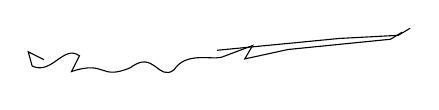
\begin{tikzpicture}[x=1cm,y=1cm]
\draw (0,0.1)--(-0.2,0.2)--(-0.15,0.02)..controls (0.1,-0.1) and (0.25,0.3)..(0.45,0.15)--(0.35,-0.05)..controls (0.8,0.1) and (0.7,-0.17)..(1.1,0)..controls (1.4,0.23) and (1.45,-0.18)..(1.65,-0.03)..controls (1.8,0.2) and (2.1,0.1)..(2.25,0.13)--(2.65,0.28)--(2.55,0.11)--(3.1,0.23)--(3.8,0.3)--(4.4,0.36)--(4.55,0.45);
\draw (2.2,0.22)--(3.75,0.37)--(4.5,0.41)--(4.65,0.5);
\end{tikzpicture}}
Soient $\underline U_0,\underline U'_0$ les ouverts de $\Psi$ induits par $\{0\}\times\Delta^1$, $\Delta^1\times\{0\}$, donc
\[
\left\{\begin{aligned}
\underline U_0&=\{0,a\},\quad\underline U'_0=\{0,b\}\\
\underline U_0\cup\underline U'_0&=\Psi,\quad\underline U_0^{\unsure{\deleted{\prime}}}\cap\underline U'_0=\{0\},
\end{aligned}\right.
\]
on aura donc
\[
\left\{\begin{aligned}
U&=\varphi^{-1}(\underline U_0),\quad U'=\varphi^{-1}(\underline U'_0)\\
U\cap U'&=\varphi^{-1}(\underline U_0\cap\underline U'_0)=\varphi^{-1}(\{0\})=X_0
\end{aligned}\right.
\]
\mspage{42}

